%%%%%%%%%%%%%%%%%%%% author.tex %%%%%%%%%%%%%%%%%%%%%%%%%%%%%%%%%%%
%
% sample root file for your "contribution" to a contributed volume
%
% Use this file as a template for your own input.
%
%%%%%%%%%%%%%%%% Springer %%%%%%%%%%%%%%%%%%%%%%%%%%%%%%%%%%


% RECOMMENDED %%%%%%%%%%%%%%%%%%%%%%%%%%%%%%%%%%%%%%%%%%%%%%%%%%%
\documentclass[graybox]{svmult}

% choose options for [] as required from the list
% in the Reference Guide

\usepackage{type1cm}        % activate if the above 3 fonts are
                            % not available on your system
%
\usepackage{makeidx}         % allows index generation
\usepackage{graphicx}        % standard LaTeX graphics tool
                             % when including figure files
\usepackage{multicol}        % used for the two-column index
\usepackage[bottom]{footmisc}% places footnotes at page bottom


\usepackage{newtxtext}       % 
\usepackage[varvw]{newtxmath}       % selects Times Roman as basic font
\usepackage{siunitx}
\usepackage{tikz}
% \usepackage[authoryear,sort]{natbib}
% \usepackage[natbib=true]{biblatex}

% see the list of further useful packages
\newcommand{\feelpp}{\texttt{Feel++}}
\newcommand{\Fluid}{\mathcal{F}} % fluid domain
\newcommand{\Real}{\mathbb{R}} % real number space
\newcommand{\Alemap}{\mathcal{A}} % Ale map
\newcommand{\ALE}{ALE} % ALE acronym
\newcommand{\Vel}{u} % fluid velocity
\newcommand{\Pres}{p} % fluid pressure
\newcommand{\Density}{\rho} % density
\newcommand{\Viscosity}{\mu} % fluid viscosity
\newcommand{\tvel}{U} % rigid body linear velocity
\newcommand{\angvel}{\omega} % rigid body angular velocity
\newcommand{\Rmat}{R} % rotation matrix frame
\newcommand{\Angle}{\theta}
\newcommand{\Inertia}{I} % inertia tensor/moment for rigid body
\newcommand{\mass}{m} % mass of the rigid body
\newcommand{\CenterMass}{x^{CM}} % center of mass of the rigid body
\newcommand{\CenterMassi}{x_{CM}^i}
\newcommand{\Solid}{\mathcal{S}} % region occupied by the body
\newcommand{\normal}{n} % outer normal to the fluid domain
\newcommand{\CompDomain}{\Fluid}
\newcommand{\dx}{\, \mathrm{d}x}
\newcommand{\Id}{\mathbb{I}}
\newcommand{\Disp}{\eta}
\newcommand{\dX}{\,\mathrm{d}X}
\newcommand{\cpp}{\texttt{C++}}
\newcommand{\R}{\mathbb{R}}
% DOUBLEHAT
\newlength{\dhatheight}
\newcommand{\hhatDS}[1]{%
	\settoheight{\dhatheight}{\ensuremath{\hat{#1}}}%
	\addtolength{\dhatheight}{-0.35ex}%
	\hat{\vphantom{\rule{1pt}{\dhatheight}}%
		\smash{\hat{#1}}}}
\newcommand{\hhatTS}[1]{%
	\settoheight{\dhatheight}{\ensuremath{\hat{#1}}}%
	\addtolength{\dhatheight}{-0.35ex}%
	\hat{\vphantom{\rule{1pt}{\dhatheight}}%
		\smash{\hat{#1}}}}    
\newcommand{\hhatS}[1]{%
	\settoheight{\dhatheight}{\ensuremath{\scriptstyle{\hat{#1}}}}%
	\addtolength{\dhatheight}{-0.175ex}%
	\hat{\vphantom{\rule{1pt}{\dhatheight}}%
		\smash{\hat{#1}}}}
\newcommand{\hhatSS}[1]{%
	\settoheight{\dhatheight}{\ensuremath{\scriptscriptstyle{\hat{#1}}}}%
	\addtolength{\dhatheight}{-0.07ex}%
	\hat{\vphantom{\rule{1pt}{\dhatheight}}%
		\smash{\hat{#1}}}}
\newcommand{\doublehat}[1]{\hat{#1}}%{\mathchoice{\hhatDS{#1}}{\hhatTS{#1}}{\hhatS{#1}}{\hhatSS{#1}}}

% in the Reference Guide

\makeindex             % used for the subject index
                       % please use the style svind.ist with
                       % your makeindex program

%%%%%%%%%%%%%%%%%%%%%%%%%%%%%%%%%%%%%%%%%%%%%%%%%%%%%%%%%%%%%%%%%%%%%%%%%%%%%%%%%%%%%%%%%

\begin{document}

\title*{Towards a computational framework using finite element methods with Arbitrary Lagrangian-Eulerian approach for swimmers with contact}
% Use \titlerunning{Short Title} for an abbreviated version of
% your contribution title if the original one is too long
\author{Luca Berti, Laetitia Giraldi, Christophe Prud'homme, Céline Van Landeghem}
% Use \authorrunning{Short Title} for an abbreviated version of
% your contribution title if the original one is too long
\institute{Luca Berti \at CNRS - Institut de Recherche Mathématique Avancée, UMR 7501 Université de Strasbourg  \email{berti@math.unistra.fr}
\and Laetitia Giraldi \at Universit\'e C\^ote d'Azur, INRIA, CNRS, Calisto team, \email{laetitia.giraldi@inria.fr}
\and Christophe Prud'homme \at Institut de Recherche Mathématique Avancée, UMR 7501 Université de Strasbourg - CNRS \email{christophe.prudhomme@math.unistra.fr}
\and Céline Van Landeghem \at Institut de Recherche Mathématique Avancée, UMR 7501 Université de Strasbourg - CNRS \email{c.vanlandeghem@unistra.fr}}
%
% Use the package "url.sty" to avoid
% problems with special characters
% used in your e-mail or web address
%
\maketitle

\abstract{Swimming involves a body's capability to navigate through a fluid by undergoing self-deformations. Typically, fluid dynamics is described by Navier-Stokes equations, and when integrated with a swimming body, it results in a highly intricate model. This paper introduces a computational framework for simulating the movement of multiple swimmers with various geometries immersed in a Navier-Stokes fluid. The approach relies on the finite element method with an Arbitrary Lagrangian-Eulerian (ALE) framework to handle swimmer displacements. Numerous numerical experiments demonstrate the adaptability of the computational framework across various scenarios.
All the implementations are made using the \feelpp\ finite element library \cite{feelpp-ref}.}




\section{Introduction}
% (LUCA) Pour tout ce que j'écris ici, il y a un paragraphe dans l'intro de ma thèse si on veut s'en inspirer
% \begin{itemize}
%         \item \textit{Paragraphe initiale}: (micro)natation (pourquoi c'est intéressant, quelles sont les particularités, citer une ou deux reviews Lauga et Elgeti, citer Purcell, medicine)
%     \item \textit{Paragraphe des méthodes numériques pour la micro-natation}: immersed boundary, boundary element and regularised kernels, resistive force theory, finite elements (il y a un paragraphe dans ma thèse. On peut prendre de là éventuellement)
%     \item \textit{Paragraphe de notre solution}: éléments finis avec ALE, contact, extension à l'élasticité avec contact aussi (possible justification du choix contre toutes les méthodes approchées, mais compétition avec immersed boundary quand-meme); le tout inséré dans une bibliothèque efficace Feel++ qui permet des simulations parallèles sur plusieurs cores
%     \item  \textit{Optimisation}: on peut rebondir sur l'efficacité de Feel++ et la précision des simulations pour dire que l'optimisation de forme ou de battement de flagelles dans la micro-natation s'est souvent concentrée sur des cas sans bord (Kenta, Yacine, Papier 87) car considérer l'influence de bords complexes ou d'autres nageurs reste compliqué. C'est aussi pour ça qu'on fait ce choix de méthode.
% \end{itemize}

% Les principaux challenges à resoudre pour faire de l'interaction fluide-structure

Swimming involves the capacity of a body to navigate through a fluid by undergoing self-deformations. Typically, the fluid dynamics is described by Navier-Stokes equations, and when coupled with a swimming body, it yields a highly intricate model. One of the main difficulties lies in the fact that the swimmers deform and move, requiring constant adjustment of the fluid domain and fluid-swimmer interface. Other difficulties come into play when accounting for obstacles, the possible presence of other swimmers, and the modeling of their interactions. These interactions are even more complex because disturbances caused by fluid agitation at one point in the domain can propagate throughout the entire domain.

% Les méthodes : Approximation : Stokes - RFT - Slender body theory - BEM (regularized stokeslet ou green kernel) - Navier-Stokes :  méthode de frontière immergée  - 


%Le problème de simuler le déplacement d'objets déformables dans un fluide peut être résolue par différentes approches. Tout d'abord, 


%For instance, in the case of microscopic bodies in fluids like water (or of macroscopic bodies in a very viscous fluid), 

The problem of simulating the motion of deformable swimmers in a fluid can be addressed through various approaches, depending on the flow regime. In the low Reynolds number limit, when the viscous effects prevail over inertial effects, as it is the case for microscopic bodies in very viscous fluids \cite{Purcell77}, it is legitimate to consider that the fluid is governed by the Stokes equations \cite{BrennerHappel65,PowersLauga09}. 

%First,
%in the case of microscopic bodies in very viscous fluids, it is well known that the locomotion of these bodies is characterized by a low Reynolds number (a dimensionless ratio between inertia effects and viscous effects) of order $10^{-6}$ \cite{Purcell77}. It is then legitimate to consider that the fluid is governed by the Stokes equations see for more details 
%(ajouter des refs Aline-Maury ?).
%\cite{AlougesGiraldi12,BrennerHappel65,PowersLauga09,LoheacMunnier12}.

%RFT
% that hydrodynamic forces applied
%to the swimmer can be derived linearly with respect to its speed
% In low Reynolds number regime, 

In this case, the hydrodynamic drag can be simplified asymptotically by employing the Resistive Force Theory \cite{GrayHanccok}, in which the hydrodynamic friction is related to the fluid velocity via an %prescribed 
anisotropic relation %operator 
depending on some parameters that account for the shape of the moving object. This approach does not require the numerical solution of the Stokes equations, but it has a
%Nevertheless, these approximations have 
very limited physical validity, often restricted to the case of very simple boundary-free domains.

%SBT
Slender body theory improves the Resistive Force Theory
to investigate the dynamics of slender particles in highly viscous flows \cite{cox1970motion, batchelor1970slender, keller1976slender,johnson1980improved}. 
This approach involves solving an integral equation which describes the effects of the fluid on the slender body. Assuming small deformations, the equilibrium of forces and torques can be expressed as a partial differential equation \cite{Gadhela_2013,  Clement_2018, Zakarya_2022}, whose solution defines the curve that describes the fiber. However, this method neglects the effects of fiber deformation on the fluid, leading to an approximation in accounting for the effects of the displacement of multiple swimmers.

%BEM (Lefebvre - Maury - Kenta)
A numerical method that is widely used in the micro-swimming community is the boundary element method, that relies on the integral formulation of the Stokes equations to determine the fluid velocity field \cite{pozrikidis1992boundary}. 
This formulation reduces the computation cost of the dynamics of the swimmer by working on the swimmer's boundary alone, which ensures significant memory savings since the fluid domain is not discretized. 
The boundary integral formulation expresses the fluid velocity at the boundary of the swimmer as a function of fluid stresses and velocities, via the fundamental solutions of the Stokes equations. Since these functions exhibit singular behaviour when the source and evaluation points are close together, a regularisation procedure needs to be employed for the numerical solution. Several solutions are possible: a regularisation of the numerical approximation of the singular integrals using a semi-analytic procedure \cite{huang_cruse} or the use of regularised kernels \cite{Fauci}. 


%citer maury lefebvre  \cite{janela2005penalty} ?


% Méthode de frontière immergée
When inertial effects become more important and the low Reynolds number assumption is no longer valid, 
it is necessary to resort to the solution of the system coupling Navier-Stokes equations with Newton's equations for rigid bodies. 
A commonly used method involves approximating the values of fluid velocity and pressure on a fixed discretization of the domain and representing the swimmers using an implicit function that parameterizes their boundaries. 
These approaches are commonly referred to Immersed Boundary Methods with level set functions describing the swimmer. 
The challenge of these methods lies in following the swimmer. 
For instance, one may use methods called CutFEM (Cut Finite Element Method), which project the swimmer's boundary onto the fixed mesh.
the CUTFEM approach in which mesh intersections are computationally costly. \cite{Monasse,Iollo,bergmann2016bioinspired,hansbo2016cut,burman2015cutfem}
%[citer Laurent Monasse, Chouly, Iollo, Giocomini Matteo]




%Maintenant si on veut calculer l'ensemble des effets physiques qui régissent de tels déplacement, il faut s'interesser à la résolution du système de Navier-Stokes couplé avec les equations de Newton pour les solides. Une des méthodes utilisées consiste à approcher les valeurs de la vitesse du fluide et de la pression sur un maillage fixe du domaine fluide et de déplacer les nageurs en utilisant une fonction implicite parametrant leurs bords.
%Ces approches sont communement conuus sous le nom de Méthodes des frontières immergées.
%La difficulté de ces méthode est de suivre le bord du nageur en fonction du temps. Par exemple, on peut utiliser des méthodes dites CUTFEM permettant de projeter à chaque iteration le bords du nageur sur le maillage fixe.

% Méthode FEM-ALE
In this chapter, we discuss an alternative method to compute the displacement of multiple deformable swimmers immersed in a Navier-Stokes fluid, which can be confined within a geometrically complex domain. This method is based on the finite element solution of the swimming problem, using the Arbitrary-Lagrangian-Eulerian description for the motion of the fluid domain.
This approach is popular in fluid-structure interaction problems \cite{chabannes2013high,pena2012high}, and it is based on a formulation of the fluid equations in an intermediate frame between the Eulerian and Lagrangian description.
A characteristic of this method is that the solutions are approximated on a mesh that deforms over time, following the deformation and movements of the swimmers.
As the immersed boundary method, it accounts for the full, non-approximated description of the fluid dynamics.
This numerical method is very versatile and it has been used in a wide variety of contexts and physical problems, and it can be easily extended to cases in which the Newtonian fluid is substituted by a complex fluid, which is often the case of biological media.

%The equations are projected on a basis of locally supported test functions, and the geometrical discretization is fitted to the moving objects. 

The structure of the chapter is the following: in Section \ref{Sec:MathModeling} the fluid, swimmer and collision models are presented. In Section \ref{Sec:NumDiscr}, the numerical discretization of the swimming problem is addressed. Finally, in Section \ref{Sec:Applications}, several numerical applications illustrate this framework.




%--------------------------------------------------------------
%------------------------------------------------------------


% Un tour d'horizon de ''Feel swimming''

% Ici on va souligner à quoi sert la librairie nageur de feel++ ?
% Quelles sont ses spécificités ?
% Présenter la méthodes et les méthodes dissidentes.

% Est-ce qu'on fait une perspectives ? 
% sinon on peut mettre un paragraphe dans l'intro avec l'elasticité.
% Optimisation de ces problemes ?


% Comment on obtient la dynamique d'un nageur en faisont une liste plus ou moins exhaustive (introduire de la bibi ici)

% Présentation de l'outil feel. Methode ALE. Avantage et ces inconvenients 

% Perspectives de feel

% organisation du papier


\section{Mathematical modeling}
\label{Sec:MathModeling}
This section details the mathematical modeling of the coupled fluid-swimmer interaction problem. A model of collision forces is also discussed, allowing to simulate swimmer-swimmer or swimmer-boundary interactions.

%\subsection{Solid swimmer in a fluid} \label{rigidbody}

% We consider solid swimmers moving in a Newtonian incompressible fluid. 
% Let's denote $d = 2$ or $d = 3$ the dimension of the time-dependent domain 
% $\Omega_t = \Solid_t \cup \Fluid_t$. 
% $\Solid_t \subseteq \Real^d$ is the region occupied by the swimmer at time $t$ and 
% $\Fluid_t \subseteq \Real^d$ the portion of $\Omega_t$ which is filled with the Newtonian fluid.
% The time $t$ is included in the interval $[0,T]$, where $T$ is the 
% final time of the simulation. 
% The fluid-swimmer interface is given by the intersection of the boundaries of the 
% two regions $\Gamma_{fsi} = \partial \Solid_t  \cap \partial \Fluid_t$.
% This subsection first describes the fluid equations, then introduces the swimmer model, 
% before explaining the fluid-swimmer coupling on $\Gamma_{fsi}$. 
\subsection{The fluid model}

%Below, we present a dynamic system that describes the dynamics of a swimmer.
%la partie fluide :
We consider Navier-Stokes equations in a moving domain to describe the motion of a Newtonian fluid medium. 
Let $\CompDomain_t\subset \R^d$, where $d=2,3$ is the dimension, denote the region occupied by the fluid at time $t$, $\mu$  the constant fluid viscosity and $\Density$ the constant fluid density. Let $\Solid_t^i \subset \R^d$ be the domain that is occupied by the body $i$, $i = 1,...,N$, where $N$ the number of bodies, of constant density $\Density_s^i$. At each time instant $t$, the fluid is in contact with the swimmers, and $\bar{\CompDomain}_{t} \cap \bar{\Solid}_t^i = \partial \Solid_t^i$.
The notations are summarized in Figure \ref{fig:swimmer-tikz}.

The velocity field $\Vel(t,x):]0,T]\times \CompDomain_t \rightarrow \R^d$ and the pressure field $\Pres(t,x):]0,T]\times\CompDomain_t \rightarrow \R$ satisfy the Navier-Stokes equations given by: 
\begin{equation}
	\begin{aligned}
		\rho\Big(\partial_t \Vel +( \Vel \cdot \nabla )\Vel \Big) - \nabla \cdot \sigma(u,p) &= f%\nabla \cdot \Stress %\nabla \Pres + \Viscosity \Delta \Vel + f 
		\quad &\text{on $ ]0,T]\times \CompDomain_t$},
		\\
		\nabla \cdot \Vel &= 0  \quad&\text{on $ ]0,T]\times \CompDomain_t$},\\
		\Vel &= \bar{\Vel}^i% U + \Omega \times(x-\bar{x}) + u_d 
		\quad &\text{on $]0,T]\times \partial \Solid_t^i$},\\
		\Vel(0,x) &= \Vel_0(x) \quad &\text{on $ \{0\}\times\CompDomain_0$},\\
		\Vel(t,x) &= h(t,x) &\text{on $ ]0,T]\times\partial\CompDomain_{t,D}$},\\
		\sigma(u,p) \normal&= g(t,x) &\text{on $ ]0,T]\times\partial\CompDomain_{t,N}$},
	\end{aligned}
	\label{Eq:NS}
\end{equation}
where $\sigma(u,p)$ is the stress tensor $-\Pres\mathbb{I} + 2 \mu D(u)$ with $D(u) = \frac{1}{2}\left(\nabla u + (\nabla u)^T\right)$ and $\bar{\Vel}^i(t,x):[0,T]\times\partial \Solid_t^i \rightarrow \R^d$ results from the interaction between the fluid and the $i$-th swimmer's body and $f(t,x):[0,T]\times\CompDomain_t \rightarrow \R^d$ represents external volume forces. The function $u_0$ is the prescribed initial condition of the system. 
\begin{figure}
    \centering
\begin{center}
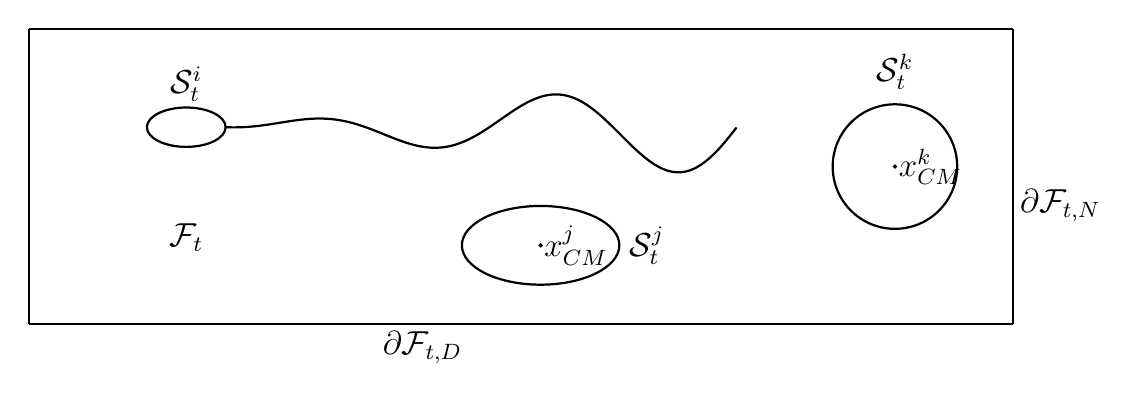
\begin{tikzpicture}

\draw[color=black,  thick] (2*5,0*3.75) -- (5*4.5,0)     ;
\draw[color=black,  thick] (2*5,1.*3.75) -- (5*4.5,1.*3.75) ;
\draw[color=black,  thick] (2*5,0) -- (2*5,1.*3.75) ;
\draw[color=black,  thick] (5*4.5,0) -- (5*4.5,1.*3.75) ;

\draw[draw=black,thick] (12,0.5*5) ellipse (0.5cm and 0.25cm);
	\begin{scope}[shift={(-3.0,0.5*5)}] \draw[draw=black,thick] plot[domain=15.5:7*pi, samples=320] (\x,{(\x-15.5)/10*sin(2*\x r)});
    \end{scope} 

\node  at (12,0.61*5) {\large{$\Solid_t^i$}};
        
\draw[color=black, thick] (15.5+1.,1.) ellipse (1*1. and 0.5*1.) ;
\node  at (15.+2.85,1.) {\large{$\Solid_t^j$}};
\draw[color=black, thick] (15.5+1.,1.) circle (0.25*1.1pt);
\node  at (15.5+1.45,1.) {\large{$x_{CM}^j$}};

\draw[color=black, thick](21,2) circle (9*2.5pt);
\node  at (21,3.2) {\large{$\Solid_t^k$}};
\draw[color=black, thick](21,2) circle (0.25*1.1pt);
\node  at (21.45,2) {\large{$x_{CM}^k$}};

\node  at (11.+1.,1.1) {\large{$\Fluid_t$}};

\node  at (23.1,1.5) {\large{$\partial \Fluid_{t,N}$}};
\node  at (15.,-0.3) {\large{$\partial \Fluid_{t,D}$}};

\end{tikzpicture}
\end{center}
   \caption{Notations for the fluid model. $\CompDomain_t$ denotes the fluid domain and $\Solid^i_t,\Solid^j_t,\Solid^k_t$ denote the swimmers and solid objects included in the fluid. $\partial \Fluid_{t,N}$ and $\partial \Fluid_{t,D}$ denote the portions of the fluid boundary where Dirichlet and Neumann boundary conditions are prescribed.}
    \label{fig:swimmer-tikz}
\end{figure}
Here $h(t,x)$ and $g(t,x)$ represent the Dirichlet and Neumann boundary conditions, prescribed on the respective portions of the fluid boundary $ ]0,T]\times\partial\CompDomain_{t,D}$ and  $ ]0,T]\times\partial\CompDomain_{t,N}$, and we have that $\partial \CompDomain_{t} = \partial\CompDomain_{t,D} \cup \partial\CompDomain_{t,N} \cup \partial \Solid_t^i$, $i=1,...,N$, for all times. 

In the case of swimming, $\bar{\Vel}^i$ can be split into two contributions. The first one is determined by the linear velocity $\tvel^i(t): [0,T]\to\R^d$ and angular velocity  $\angvel^i(t):[0,T]\to \R^{d^*}$ of the swimmer around its center of mass $\CenterMassi$, where $d^*=1$ if $d=2$ and $d^*=3$ if $d=3$, while the second one is given by the deformation velocity of the solid $\Vel_d^i$, if present. The function $\bar{u}^i$ then becomes $\bar{\Vel}^i(t,x) = \tvel^i(t) + \angvel^i(t)\times (x-\CenterMassi)+ \Vel_d^i(t)$.

% Let's denote $\Vel : [0,T] \times \Fluid_t \mapsto \Real^d$ the fluid velocity, 
% $\Pres : [0,T] \times \Fluid_t \mapsto \Real$ the hydrostatic pressure, and 
% $\mu, \Density_f \in \Real^{+} $ the fluid viscosity and constant density. 
% To have a common description of the hydrodynamics and the rigid swimmer dynamics, 
% the fluid motion is described in the Arbitrary-Lagrangian-Eulerian (ALE) formalism. 
% The reference domain $\Fluid_0$ is mapped to the current fluid domain $\Fluid_t$ using 
% the ALE map $\Alemap_t : \Fluid_0 \rightarrow \Fluid_t$, defined as 
% $\Alemap_t(X) = \Alemap(t,X) = X + \phi(t,X)$, where $\phi_t$ the displacement of the domain.
% The change from the Eulerian frame, which is generally used in fluid mechanics, 
% to the ALE formalism introduces additional terms for the time derivative 
% in the momentum equation : 
% $\partial_t \Vel = \partial_t \Vel |_\Alemap - ( \Vel_\Alemap  \cdot \nabla )\Vel$.
% The first term of the \ALE\ derivative corresponds 
% to the time variation of the fluid velocity as seen in the \ALE\ frame, 
% while the second contains the relative velocity of the moving domain. 
% The Navier-Stokes equations in the \ALE\ frame, describing the velocity $u$ and pressure $p$, are given by: 

% \begin{equation}
% 	\begin{aligned}
% 		\Density_f\partial_t \Vel |_\Alemap+ \Density_f \Big((\Vel - \Vel_\Alemap)\cdot \nabla\Big) \Vel &= -\nabla \cdot \sigma + F, \qquad & \mbox{in $\Fluid_t$,}\\
% 		\nabla \cdot \Vel &=0, \qquad & \mbox{in $\Fluid_t$},
% 	\end{aligned}
% 	\label{eq:fluid}
% \end{equation}

% where $\sigma \in \mathcal{M}_d(\Real)$ is the fluid stress tensor and $F \in \Real^d$ 
% are the external volume forces. 

\subsection{The swimmer model}

% The propulsion of the solid swimmer is described by a deformation velocity $u_d(t,X) : [0,T] \times \Solid_0 \rightarrow \Real^d$ 
% defined on the swimmer's boundary $\partial \Solid_0$. 
% We consider swimmers whose deformation velocity is expressed by an analytical formula, fixing for instance a velocity field tangent to $\partial \Solid_0$, see section \cite{}, or the relative velocity between the parts of the articulated swimmers.
% The motion of the swimmer is not only influenced by this interaction with the fluid but also by a rigid-body contribution due to external forces $F_e \in \Real^d$ and torques $T_e \in \Real^{d^{*}}$, where $d^{*} = 1$ if $d = 2$, else $d^{*} = 3$. The rigid-body contribution is described by the motion of the swimmer's center of mass,
% given by the Newton equation, and the rotation matrix between its local frame and the global frame, which evolves according to the Euler equation.
% Let's denote $\tvel: [0,T] \to \Real^d$ the translational velocity of the swimmer and $\angvel:[0,T]\to \Real^{d^*}$ its angular velocity. 

The swimmer's motion is either a result of its deformation, which generates hydrodynamic forces that are then translated into rigid movement through Newton's laws, or external forces such as gravity or collision forces. 

Let us define the mass of the $i$-th swimmer be given by  $\mass^i = \int_\Solid \Density_{\Solid}^i$ %, let $\CenterMassi = \frac{1}{\mass^i} \int_{\Solid^i} \Density_{\Solid}^i x$ be its center of mass, 
and $\Inertia^i = \int_{\Solid^i} \Density_{\Solid}^i (x-\CenterMassi) \otimes (x-\CenterMassi)$ 
its positive definite and symmetric inertia tensor. 
The Newton and Euler equations describing the rigid body velocities $\tvel^i$ and $\angvel^i$ read:
\begin{equation}
	\begin{aligned}
		\mass^i \frac{d}{dt}\tvel^i &= F_e^i -\int_{\partial \Solid^i} \sigma \normal \,\textrm{ds},\\
		\frac{d}{dt}(\Rmat \Inertia^i \Rmat^T \angvel^i) &= T_e^i -\int_{\partial \Solid^i} \sigma \times (x-\CenterMassi)\,\textrm{ds}, 
	\end{aligned}
	\label{Eq:RB}
\end{equation}

where $\normal$ is the unit outward normal to $\partial \Solid^i$. The rotational speed $\angvel^i_k$ is linked with the orientation of the swimmer using

\begin{equation*}
	\begin{aligned}
		\frac{d}{dt} \Angle_k &= \angvel^i_k, \quad \text{for $k \in \{x,y,z\}$},\\
		\Rmat &=\Rmat_z(\Angle_z)\Rmat_y(\Angle_y)\Rmat_x(\Angle_x),
	\end{aligned}
\end{equation*}
where $R_k(\Angle_k)$ denotes the rotation matrix around axis $k \in \{x,y,z\}$ of 
angle $\Angle_k$. If $d=2$, $R(\theta)$ has the form: 
\begin{equation*}
	\begin{aligned}
		\Rmat(\Angle) &= \begin{bmatrix}
			\cos(\Angle) & \sin(\Angle)\\
			-\sin(\Angle) & \cos(\Angle)
		\end{bmatrix}.
	\end{aligned}
\end{equation*}
While in three dimensions:
$$	
	\Rmat_z(\Angle_z) = \begin{bmatrix}
		\cos(\Angle_z) & -\sin(\Angle_z) & 0\\
		\sin(\Angle_z) & \cos(\Angle_z)& 0 \\
		0& 0 & 1
	\end{bmatrix},
	\Rmat_y(\Angle_y) = \begin{bmatrix}
		\cos(\Angle_y) &0 & \sin(\Angle_y) \\
		0& 1& 0\\
		-\sin(\Angle_y) & 0& \cos(\Angle_y)
	\end{bmatrix},\\
$$
$$
	\Rmat_x(\Angle_x) = \begin{bmatrix}
		1 & 0 & 0\\
		0 &\cos(\Angle_x) & -\sin(\Angle_x) \\
		0 &\sin(\Angle_x) & \cos(\Angle_x) 
	\end{bmatrix}.
$$
The angle $\Angle$ belongs to  $\Theta$, with $\Theta = [-\pi,\pi]$ if $d=2$, 
or $\Angle_k \in \Theta$, for $k=x,y,z$, $\Theta=[-\pi,\pi]\times[0,\pi]\times[0,\pi/2]$ if $d=3$.

Equations \eqref{Eq:RB} correspond to the balance of forces and torques applied to each swimmer, stating that non-zero net contributions from fluid stresses $\sigma n$ or additional external forces $F_e^i$ and torques $T_e^i$ lead to velocity variations.

% \paragraph{The fluid-solid interaction}

% On the fluid-swimmer interface $\Gamma_{fsi}$ three additional conditions are prescribed. The kinematic condition imposes the continuity of the velocities:
% \begin{equation}
% 	\Vel = \tvel + \angvel \times (x-\CenterMass) + R(t) u_d(\Alemap_t^{-1}(x)) \quad \text{on $\Gamma_{fsi}$}.
% \end{equation}

% The dynamic condition forces the transmission of fluid forces and torques to the solid swimmer, which is ensured by the Newton and Euler equations in \eqref{Eq:RB}. Finally, the geometric condition prescribes that the time evolution of the fluid boundary $\partial \Fluid_t$ corresponds to the time evolution of the solid boundary $\partial \Solid_t$. Thus, the displacement $\phi_t$ of the \ALE\ map is solution of the following elliptic equation:  
% \begin{equation}
% 	\begin{aligned}
% 		\nabla \cdot([1+\tau(X)]\nabla_X \phi(t,X)) &= 0 \quad &\text{in $\Fluid_0$}, \\
% 		\phi(t,X) &= g(t,X) \quad &\text{in $\partial \Fluid_0$}, 
% 	\end{aligned}
% 	\label{Eq:ALE}
% \end{equation}
% where $g(t,X)  = \int_0^t \tvel + \angvel \times(X-X^{CM})$ is the rigid displacement 
% of $\Solid_t$ and $\tau(X)$ is a space-dependent coefficient, whose definition is given in \cite{}.


\subsubsection{Collision model} 
\label{rigidcollision}

In this subsection, we describe how a swimmer's collisions with solid obstacles, other swimmers (as active particles), and the boundaries of the fluid domain are handled. Our model is based on a short-range contact-avoidance repulsive force introduced by R. Glowinski in \cite{glowinski}, for which a collision zone of width $\rho$ is defined in which the forces are activated.
In equation \eqref{Eq:RB}, the external force and torque terms $F_e^i$ and $T_e^i$ summarize the physical interactions occurring when the distances $d_{ij}$ and $d_{i}$ between swimmer $i$ and another body $j$, or between swimmer $i$ and the domain boundary $\partial \Fluid_t$, are smaller than the width $\rho$ of the collision zone.  
The definition of the collision force for a swimmer-swimmer or swimmer-boundary pair is given by: 

$$
\overrightarrow{F_{ij}} = - \epsilon A  \overrightarrow{X_i X_j }  1_{d_{ij} \leq \rho}, \qquad
\overrightarrow{F_{i \partial \Fluid_t}} = - \epsilon' A \overrightarrow{X_i X_{\partial \Fluid_t} }  1_{d_{i} \leq \rho}.
$$

Both equations contain an activation term $A$, depending on the type of the swimmer under consideration.  The vector connecting the contact points $X_i, X_j$ or $X_i, X_{\partial \Fluid_t}$
gives the direction of the force, and the stiffness parameters $\epsilon$ and $\epsilon'$ determine the force intensity. As a general rule, the force magnitude increases as the distance decreases. Finding the optimal values for $\epsilon$ and $\epsilon'$ is not trivial, since their values depend on fluid and swimmer properties.   

The total repulsion force applied on $\Solid^i$ is defined by:
$$
\overrightarrow{F_i} = \sum_{(i,j)|d_{ij} \leq \rho} \overrightarrow{F_{ij}} +  \sum_{i | d_i \leq \rho} \overrightarrow{F_{i \partial \Fluid_t}},
$$
where the first sum runs over all the body pairs $(i,j)$ such that $d_{ij}\le \rho$, and the second sum runs over all body-boundary pairs such that $d_{i}\le \rho$.

Force $\overrightarrow{F_i}$ leads to body rotations via its associated torque, defined by: 
$$
\overrightarrow{T_i} = - \overrightarrow{x_{CM}^i X_i} \times \overrightarrow{F_i},
$$
where $\overrightarrow{x_{CM}^i X_i}$ connects the center of mass of $\Solid^i$ and the contact point $X_i$ where $\overrightarrow{F_i}$ is applied.

The total repulsion force $\overrightarrow{F_i}$ and the external associated torque $T_i$ are added to  $F_e^i$ and $T_e^i$ in the Newton equation \eqref{Eq:RB}, thus modifying the trajectory of the swimmer.  

% Resumé article collision
% \subsection{Elastique}
% Luca + Celine
% Papier Burman
% Luca - notes
% We consider only the no-slip formulation [because the stresses in the slip case are a bit more complicated, and] in the Stokes regime we suppose that the fluid is moving with the solid. In any case, we refer the reader to the paper for the slip formulation. The variational formulation of the problem in equation (24), where a Nitsche-like term appears only on the solid side (since only the normal component of the $w$ test function is considered). Equation (41) considers the generalized formulation from Chouly with $\theta$, adds consistency terms with time derivatives, and tests against variants of $\sigma_n$. However, their numerical results are restricted to the case $\theta=0$, so maybe we should restrict ourselves to that too?

\section{Numerical discretization}
\label{Sec:NumDiscr}

\subsection{The Arbitrary-Lagrangian-Eulerian formalism}
% Introduire le framework ALE --- DONE @LUCA
We rewrite the fluid problem under consideration, defined on a time-dependent domain, using the Arbitrary-Lagrangian-Eulerian (\ALE) formalism, which decouples the evolution of the computational domain from the evolution of the underlying fluid continuum. 
Let $\CompDomain_t$ be the computational domain where the fluid equations are solved at time $t$. We define the \ALE\ maps $\Alemap_t:\CompDomain_0 \to \CompDomain_t$ as the family of smooth and bijective functions that describe the evolution of the computational domain. These functions are defined through the extension of the displacement field at the boundary of the computational domain $\partial \CompDomain_t$ to the interior of $\CompDomain_t$. For instance, if $\bar{\phi}_t:\partial \CompDomain_0 \to \partial \CompDomain_t$ is the boundary displacement, a possible definition of the \ALE\ maps is $\Alemap_t(X) = X + \phi_t(X)$, for $X \in \CompDomain_0$, where $\phi_t(X)$ is the extension of $\bar{\phi}_t$ via
\begin{equation}
	\left\{
	\begin{aligned}
		&\nabla \cdot((1+\tau(X))\nabla \phi_t(X)) = 0, \quad &\text{on $\CompDomain_0$},\\
		&\mathcal{\phi}_t= \bar{\phi}_t, &\text{on $\partial \CompDomain_0$},
	\end{aligned}
	\right.
 \label{Eq: VarFormALE}
\end{equation}
where $\tau(X)$ acts as a space-dependent diffusion coefficient influencing the regions where larger displacements are localised.

The time derivative of $\Vel$ in the \ALE\ frame can be expressed as a function of its Eulerian time derivative $\partial_t \Vel$ and the \ALE\ velocity $\Vel_{\mathcal{A}}(t,X)=\frac{\partial x}{\partial t}(t,\Alemap_t^{-1}(x))$, $X \in \CompDomain_0$, which is the velocity of the moving domain:
\begin{equation}
\frac{\partial \Vel}{\partial t} \Big|_{\Alemap_t}(t,x)=\Vel_{\mathcal{A}} \cdot \nabla \Vel + \partial_t \Vel, \quad \text{$ x \in \CompDomain_t$}.
\end{equation}


% discretisation ALE --- to rephrase & correct @LUCA
In the discrete setting, it is not guaranteed that displacing the mesh according to the solution of \eqref{Eq: VarFormALE} always produces a valid triangulation: large displacements could lead to element inversions.
In order to prevent these problems, mesh quality measures \cite{Field2000} are used to assess the validity of the triangulation: if the mesh deformation is ``small'' and the mesh quality remains above a predefined threshold, the domain is deformed according to the \ALE\ map; if the minimum of the mesh quality field falls below the threshold, the resulting mesh deformation is not viable and a remeshing procedure is applied before the \ALE\ map.

In our case, the discrete \ALE\ maps are computed by solving equation \eqref{Eq: VarFormALE} with piece-wise linear continuous finite elements. The spaces where the numerical solution and the test functions are chosen are defined as
\begin{equation}
	\begin{aligned}
		X_{\bar{\phi}}^h &= \{  \phi \big| \phi \in [H^1(\CompDomain^h_{0})]^d\cap [\mathbb{P}^1(\CompDomain^h_{0})]^d, \phi=\bar{\phi} \text{ on $\partial \CompDomain^h_{0}$}\},\\
		X_0^h &= \{  \phi \big| \phi \in [H^1_0(\CompDomain^h_{0})]^d\cap [\mathbb{P}^1(\CompDomain^h_{0})]^d\},
	\end{aligned}
\end{equation}
and the solution of the variational problem 
	\begin{equation}
		\begin{aligned}
			&\int_{\CompDomain^h_{0}} (1+\tau(X))\nabla \phi^{t_{n+1}}_h (X)  : \nabla v \,\dx= 0, \qquad &\text{$\forall v \in X_0^h$},
			\\
			&\mathcal{\phi}_h^{t_{n+1}}= \bar{\phi}^{t_{n+1}}, &\text{on $\partial \CompDomain^h_{0}$}.
		\end{aligned}
	\end{equation}
defines the new computational domain as $\CompDomain^h_{t_{n+1}}=\Alemap_h^{t_{n+1}}(\CompDomain^h_{0})$, where $\Alemap_h^{t_{n+1}}(X) = X + \phi_h^{t_{n+1}}(X)$. 
Here $\bar{\phi}^{t_{n+1}}(X) = \int_{0}^{t_{n+1}}\tvel + \angvel\times(X+\phi^{t_n}(X)-X^{CM}_{0}-\phi^{t_n}(X^{CM}_{0})) + Ru_d(t,X)\, \mathrm{d}t$ is the accumulated body displacement and $\tau$ is a piecewise constant coefficient, defined on each element $e$ of the domain's discretization as $ \tau\big |_e=(1-V_{min}/V_{max})/(V_e/V_{max})$, where $V_{max}$, $V_{min}$  and $V_e$ are the volumes of the largest, smallest and current element of the domain discretization \cite{kanchi_3d_2007}.
The time integration of $\bar{\phi}^{t_{n+1}}$  is performed in two steps: first, the contributions coming from the linear velocity are integrated to compute the new center of mass $\bar{\phi}_1^{t_{n+1}}(X^{CM}_0) $ as
\begin{equation}
	\begin{aligned}
		\theta_{n+1}&= (t_{n+1}-t_n)\angvel^n + \theta_{n}, \quad R^{n+1} = R(\theta_{n+1}),\\
		\bar{\phi}_1^{t_{n+1}}(X) &= (t_{n+1}-t_n)\tvel^n + \phi^{t_{n}}(X) + R^{n+1}\int_0^{t_{n+1}} u_d(t,X)\, \mathrm{d}t;
	\end{aligned}
	\label{Eq:discDisp1}
\end{equation}
and then the orientation of the body is computed using the new center of mass
\begin{multline}
	\bar{\phi}^{t_{n+1}}(X) \approx  R(\theta_{n+1}) (X+\phi_1^{t_{n+1}}(X)-\phi_1^{t_{n+1}}(X_{CM}^{0})) + \phi_1^{t_{n+1}}(X_{CM}^0)-X,
	\label{Eq:discDisp2}
\end{multline}
and few fixed point iterations are performed at each time step to ensure the convergence of the body's position.


\subsection{Discretization of the fluid problem}
% discretisation des equations navier-stokes + newton
% Let $\mathcal{T}_0$ be the triangulation discretizing the fluid domain $\Fluid_0$ at time $t=0$. The triangulation follows the motion of the computational domain $\CompDomain_t$, as described by the \ALE\ maps $\Alemap_t$, according to a discrete approximation of the latter, that we denote $\Alemap_h^t$, and for each $t_n$, $0\le n \le n_T$,  we define the triangulation $\mathcal{T}_{t_n} = \Alemap_h^{t_n} (\mathcal{T}_0)$. 

Let $\Vel_h^n$ and $\Pres_h^n$ denote the discrete approximations of the velocity and pressure fields at time $t_n$. Since the domain is time dependent, the functional spaces are time dependent as well via the discrete \ALE\ maps:
\begin{equation}
	\begin{aligned}
		V_h^t &= \{v: \CompDomain_t \to \mathbb{R}^d, \, v = \hat{v} \circ (\mathcal{A}_h^t)^{-1}, \, \hat{v} \in [H^1(\CompDomain_0)]^d \cap [\mathbb{P}_N(\CompDomain_0)]^d  \}, \\
		Q_h^t &= \{\Pres : \CompDomain_t \to \mathbb{R}, \, \Pres = \hat{\Pres} \circ (\Alemap_h^t)^{-1}, \, \hat{\Pres} \in\mathbb{P}_{N-1}(\CompDomain_0) \}.
	\end{aligned}
	\label{Eq:FEMspace}
\end{equation}
We choose the Taylor-Hood finite element spaces $V_h^t -Q_h^t $ with $N=2$ for our finite element simulations.
The discrete variational formulation of the Navier-Stokes equations in moving domain at time $t_{n+1}$ requires finding $(\Vel_h^{n+1}, \Pres_h^{n+1}) \in V_h^{t_{n+1}} \times Q_h^{t_{n+1}}$, $(\tvel^{n+1},\angvel^{n+1})\in \mathbb{R}^d\times \mathbb{R}^{d^*}$ such that, for all $(\tilde{\Vel},\tilde{\Pres}) \in V_{h}^{t_{n+1}} \times Q_h^{t_{n+1}}, (\tilde{\tvel},\tilde{\angvel}) \in \mathbb{R}^d\times \mathbb{R}^{d^*}$

\begin{multline}
	\int_{\CompDomain_{t_{n+1}}} \rho_f\partial_t \Vel_h^{n+1}|_\Alemap  \cdot \tilde{\Vel} + \int_{\CompDomain_{t_{n+1}}} \rho_f((\Vel_h^{n+1}-{\Vel_{\mathcal{A}}}_h^{n+1} )\cdot \nabla_x u_h^{n+1}) \cdot \tilde{\Vel}+
 \\
 + \frac{d[R(t)IR(t)^T\angvel]}{dt}^{n+1} \cdot \tilde{\angvel}+m\frac{d\tvel}{dt}^{n+1}\cdot \tilde{\tvel} +
	\\ + 
	2\mu\int_{\CompDomain_{t_{n+1}}} [(\nabla \Vel_h^{n+1} + \nabla \Vel_h^{n+1,T})] :  [(\nabla \tilde{\Vel} + \nabla \tilde{\Vel}^T)]  \, dx  %-\int_{\partial \Solid^h} (-\Pres_h^{n+1} \mathbb{I} + 2\mu D(\Vel_h^{n+1})) \normal \cdot v\, dS
	-\int_{\CompDomain_{t_{n+1}}} \Pres_h^{n+1} \nabla_x\cdot \tilde{\Vel} = \int_{\CompDomain_{t_{n+1}}} f^{n+1} \cdot \tilde{\Vel},
	\label{Eq:discrete-var_form}
\end{multline}
\begin{equation}
	\int_{\CompDomain_{t_{n+1}}} \tilde{\Pres} \nabla_x\cdot \Vel_h^{n+1} = 0.
	\label{Eq:discrete-var_form2}
\end{equation}
Following \cite{maury}, let us now denote the degrees of freedom that belong to the boundary of the rigid body by the subscript $\Gamma$ as $\Vel_\Gamma, \Pres_\Gamma$ and the others by the subscript $I$ as $\Vel_I, \Pres_I$.

The boundary terms $	\int_{\partial \Solid} (-\Pres\mathbb{I} + 2\mu D(\Vel)) \normal \cdot\tilde{\Vel}\, dS $ are never computed in the assembly of the system matrix: 
instead of building the finite element basis $(\tilde{\Vel},\tilde{\tvel},\tilde{\angvel}) \in [H^1(\CompDomain_{t_{n+1}})]^d \times \mathbb{R}^d \times \mathbb{R}^{d^*}$ that satisfies boundary conditions $\Vel = \tvel+ \angvel \times (x-x_{CM}) + u_d$ on  $\partial \Solid$, we discretize equations \eqref{Eq:discrete-var_form}-\eqref{Eq:discrete-var_form2} using the unconstrained basis, getting the following saddle point problem
\begin{equation}
	\begin{bmatrix}
		A_{II} & A_{I\Gamma} & 0 & 0 & B_{I}^T  \\
		A_{\Gamma I} & A_{\Gamma \Gamma}  & 0 & 0 & B_{\Gamma}^T\\
		0 & 0 & T
		& 0 & 0 \\
		0 & 0 & 0& M
		& 0\\
		B_I & B_\Gamma & 0 & 0 & 0   \\
	\end{bmatrix}
	\begin{bmatrix}
		\Vel_I \\ \Vel_\Gamma \\ \tvel \\ \angvel \\ \Pres 
	\end{bmatrix} 
	= 
	\begin{bmatrix}
		0 \\
		0\\
		0
		\\
		0
		\\
		0
	\end{bmatrix},
	\label{Eq:flu-rig-block}
\end{equation} 
where
\begin{multline*}
	A_{JK} =	\int_{\CompDomain_{t_{n+1}}} \rho_f(\partial_t u_h^{n+1}|_\Alemap )_J \cdot \tilde{\Vel_K} + \int_{\CompDomain_{t_{n+1}}}\rho_f ((\Vel_h^{n+1}-{\Vel_{\mathcal{A}}}_h^{n+1} )\cdot \nabla_x u_h^{n+1})_J \cdot \tilde{\Vel_K} + \\
	2\mu\int_{\CompDomain_{t_{n+1}}} D(\Vel_h^{n+1})_J	: D(\tilde{\Vel_K}) \, dx, \quad \text{for $J,K \in \{I,\Gamma\}$} 
\end{multline*}
\begin{equation*}
	B_I = -\int_{{\CompDomain_{t_{n+1}}} } \Pres_{h}^{n+1} \nabla\cdot \tilde{\Vel_I} \, dx \qquad  B_\Gamma =  -\int_{{\CompDomain_{t_{n+1}}} } \Pres_{h}^{n+1} \nabla\cdot \tilde{\Vel_\Gamma} \, dx,
\end{equation*}
\begin{equation*}
	T = m\mathbb{I}, \qquad M = R^nI^n(R^n)^T.
	%\tilde{M}_\Pres= - \int_{\partial P} -\Pres \vec{n} \times (x-\CenterMass)\cdot \tilde{\angvel}\, dS.
\end{equation*}
Then, the operator 
\begin{equation*}
	P = \begin{bmatrix}
		\mathbb{I} &  0 & 0 \\
		0 & \tilde{P}_\tvel & \tilde{P}_\angvel\\
		0 &  \mathbb{I} & 0\\
		0 & 0 & \mathbb{I}
	\end{bmatrix}, 
\end{equation*}
that satisfies the equation
\begin{equation*}
 (\Vel_I,\Vel_\Gamma,\tvel,\angvel)^T =	P(\Vel_I,\tvel,\angvel)^T + R(t)u_d
\end{equation*}
is built, as it performs the change of finite element basis from the standard Lagrange basis to the one satisfying $\tilde{\Vel} = \tilde{\tvel} + \tilde{\angvel}\times (x-\CenterMass)$ on $\partial \Solid$. In the previous matrix, $\tilde{P}_\tvel$ and $ \tilde{P}_\angvel$ are the interpolation operators that enable the expression of $u_\Gamma$ as a function of $\tvel$ and $\angvel$. 

After extending the operator $P$ to $\mathcal{P}$ in order to include the pressure degrees of freedom,
\begin{equation*}
	\mathcal{P} =
	%	\begin{bmatrix}
	%		I & 0 & 0 & 0 & 0\\
	%		0 &  0 & \tilde{P}_\tvel & \tilde{P}_\angvel & 0\\
	%		0 & 0 & I & 0 & 0\\
	%		0 & 0 & 0 & I & 0\\
	%		0 & 0& 0& 0& I
	%	\end{bmatrix},
	\begin{bmatrix}
		\mathbb{I} &  0 & 0 & 0\\
		0 &\tilde{P}_\tvel & \tilde{P}_\angvel & 0\\
		0 &\mathbb{I} & 0 & 0\\
		0 &0 & \mathbb{I} & 0\\
		0 &0& 0& \mathbb{I}
	\end{bmatrix},
\end{equation*}
it is possible to compute the matrix expressing the coupled fluid-rigid body problem by conjugation with $\mathcal{P}$ 
\begin{equation*}
	\mathcal{P}^T \begin{bmatrix}
		A_{II} & A_{I\Gamma} & 0 & 0 & B_{I}^T  \\
		A_{\Gamma I} & A_{\Gamma \Gamma}  & 0 & 0 & B_{\Gamma}^T\\
		0 & 0 & T & 0 & 0 \\
		0 & 0 & 0& M 
		& 0\\
		B_I & B_\Gamma & 0 & 0 & 0   \\
	\end{bmatrix} \mathcal{P} = 
	\begin{bmatrix}
		A_{II}& A_{I\Gamma}\tilde{P}_\tvel   & A_{I\Gamma} \tilde{P}_\angvel   & B_{I}^T  \\
		\tilde{P}_\tvel^T A_{\Gamma I}  & \tilde{P}_\tvel ^T A_{\Gamma \Gamma} \tilde{P}_\tvel + T & \tilde{P}_\tvel ^T A_{\Gamma \Gamma} \tilde{P}_\angvel & \tilde{P}_\tvel^TB_{\Gamma}^T\\
		\tilde{P}_\angvel^T A_{\Gamma I}  & \tilde{P}_\angvel ^T A_{\Gamma \Gamma} \tilde{P}_\tvel & \tilde{P}_\angvel ^T A_{\Gamma \Gamma} \tilde{P}_\angvel + M& \tilde{P}_\angvel^TB_{\Gamma}^T\\
		B_I   & B_\Gamma\tilde{P}_\tvel  &  B_\Gamma\tilde{P}_\angvel & 0   \\
	\end{bmatrix},
\end{equation*}
and the right-hand side of the coupled problem by multiplying it by $\mathcal{P}^T$ and by adding the term depending on $\Vel_d$
\begin{equation}
	\mathcal{P}^T 	\begin{bmatrix}
		0 \\
		0\\
		F_e
		\\
		M_e
		\\
		0
	\end{bmatrix} - \mathcal{P}^T \begin{bmatrix}
		A_{II} & A_{I\Gamma} & 0 & 0 & B_{I}^T  \\
		A_{\Gamma I} & A_{\Gamma \Gamma}  & 0 & 0 & B_{\Gamma}^T\\
		0 & 0 & T & 0 & 0 \\
		0 & 0 & 0& M 
		& 0\\
		B_I & B_\Gamma & 0 & 0 & 0   \\
	\end{bmatrix}\begin{bmatrix}
		0 \\
		R(t)u_d \cdot \Alemap^{-1}_t\\
		0
		\\
		0
		\\
		0
	\end{bmatrix}.
\end{equation}


\subsection{Collision model}

\begin{figure}
    
\begin{center}
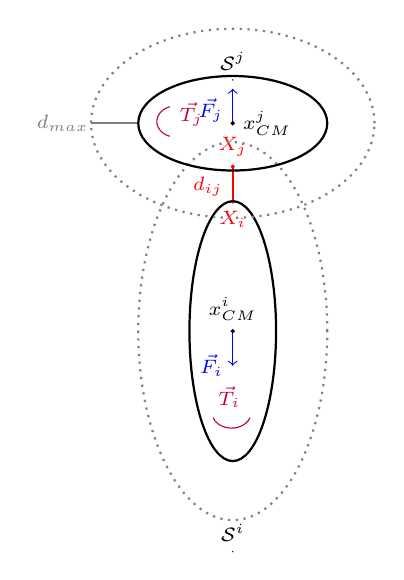
\begin{tikzpicture}

\draw[color=red, thick](0,1.5*1.1) -- (0,1.9*1.1) node[font = \scriptsize, anchor = north east] {$d_{ij}$}  ;
\draw[color=red, thick](0,1.5*1.1) circle (0.25*1.1pt) node[font = \scriptsize, anchor = north] {$X_i$};
\draw[color=red, thick](0,1.9*1.1) circle (0.25*1.pt) node[font = \scriptsize, anchor = south] {$X_j$};

\draw[color=gray, thick](-1*1.2,2.4*1.1) -- (-1.5*1.2,2.4*1.1) ;

\node[font = \scriptsize,color=gray]  at (-1.8*1.2,2.4*1.1) {$d_{max}$};


\draw[color=blue, thin,->](0,0) -- (0,-0.4*1.1)  node[font = \scriptsize, anchor = east] {$\vec{F_i}$} ;
\draw[color=blue, thin,->](0,2.4*1.1) -- (0,2.8*1.1)node[font = \scriptsize, anchor = north east] {$\vec{F_j}$}  ;

\draw[color=black, thin](0,2.9*1.1) circle (0.0001) node[font = \scriptsize, anchor = south ] {$\Solid^j$} ;
\draw[color=black, thin](0,-2.8) circle (0.0001) node[font = \scriptsize, anchor = south] {$\Solid^i$} ;
\draw[color=purple, thin] (-0.8,2.85) arc(110:250:0.25 and 0.2)node[font = \scriptsize, anchor = south west] {$\vec{T_j}$} ;

\draw[color=purple, thin] (-0.25,-1.1) arc(200:340:0.25 and 0.2)node[font = \scriptsize, anchor = south east] {$\vec{T_i}$} ;


\draw[color=black, thick] (0,0) ellipse (0.5*1.1 and 1.5*1.1) ;
\draw[color=gray, thick, dotted] (0,0) ellipse (1*1.2 and 2*1.2);
\draw[color=black, thick](0,0.) circle (0.25*1.1pt) node[font = \scriptsize, anchor = south] {$x_{CM}^i$};


\draw[color=black, thick] (0,2.4*1.1) ellipse (1*1.2 and 0.5*1.2);
\draw[color=gray, thick, dotted] (0,2.4*1.1) ellipse (1.5*1.2 and 1.*1.2);
\draw[color=black, thick](0,2.4*1.1) circle (0.25*1.1pt) node[font = \scriptsize, anchor = west] {$x_{CM}^j$};

\end{tikzpicture}
\end{center}
   \caption{Notations for the collision model.  $\Solid^i,\Solid^j$ denote the solid objects, $d_{ij}$ the distance between the two bodies, and
$d_{max}$ the threshold distance for the narrow-band fast marching method. $F_i,F_j$ and $T_i, T_j$ denote the collision forces and torques.  }
    \label{fig:collision-tikz}

\end{figure}


% force de coliisions
The collision detection algorithm, which identifies the pairs of swimmers that are actually interacting as those whose surfaces are less than $\rho$ units apart, is based on the computation of distance functions. Figure \ref{fig:collision-tikz} shows the different notations. 
%One of the difficulties of taking into account the interaction effects is the computation of the distance functions between moving bodies and fixed boundaries.
At each time instant, the distances $d_{ij}$ between the surfaces of two swimmers $\Solid^i$ and $\Solid^j$, $i \ne j$ are needed to determine if collision forces need to be activated. In order to compute them, a narrow-band variant of the fast marching method is used. 
%The fast marching method is based on a level set algorithm introduced by J.A Sethian in \cite{sethian}. 

When applied to a body $\Solid^i$, the  fast marching algorithm \cite{sethian} yields the distance field $D_i$ from $\Solid^i$ the to rest of the domain. However, since we are interested in the evaluation of the distance function in a small neighbourhood of $\Solid^i$, we employ a narrow-band approach that only computes $D_i$ close to $\partial \Solid^i$. This choice accelerates considerably the computations, especially in three dimensions, and is also suitable for parallel execution.
%To accelerate this method, which is computationally expensive, especially in three dimensions, we develop the narrow-band approach, designed to run in parallel. This approach calculates the distance field only in a restricted neighborhood of $\partial \Solid^i$. 

The size of the neighborhood is set to a predefined threshold $d_{max}$, defined as a function of $\rho$. Upon reaching the threshold distance $d_{max}$, the narrow-band 
approach assigns a default value $\delta$ to the distance field, corresponding to the maximum value reached:
\begin{center}
	\begin{equation*}
		D_i^{NB} = \left\{\begin{array}{rcl}
		0 \;, \quad &\mbox{on }& \partial \Solid^i , \\
		D_i \;, \quad &\mbox{for }& D_i \leq d_{max} ,\\
		\delta\;, \quad &\mbox{elsewhere}&   .
		\end{array}\right.\;
	\end{equation*}
\end{center}

Using the two distance fields $D_i$ and $D_j$, the distance $d_{ij}$ is described by:
$$
d_{ij} = ||\arg\min_{x \in \partial \Solid^j}  D_i^{NB}(x) - \arg\min_{x \in \partial \Solid^i} D_j^{NB}(x)||_2. 
$$
The boundary points $X_i = \arg\min_{x \in \partial \Solid^i} D_j^{NB}(x)$ and $X_j = \arg\min_{x \in \partial \Solid^j}  D_i^{NB}(x)$ 
give the contact points of the swimmers $\Solid^i$ and $\Solid^j$, i.e., the coordinates 
of the points where they will interact. 

Similarly to the case of two interacting bodies, it is possible to compute the distance between a swimmer and the boundaries of the fluid domain: 
$$
d_{i} = ||\arg\min_{x \in \partial \Fluid_t} D_i^{NB}(x) - \arg\min_{x \in \partial \Solid^i} D_{\Fluid_t}^{NB}(x)||_2 \mbox{,}
$$
where $D_{\Fluid_t}^{NB}$ represents the distance field obtained by applying the fast marching method 
to the portion of the domain boundary $\partial \Fluid_t \backslash ( \cup_i \partial \Solid^i ) $. 



\section{Applications}
\label{Sec:Applications}
% squirmers (resumé squirmer)
% contact de squirmers
% contact elastique pas dans le fluide
% 

We present numerical simulations of swimming micro-organisms to illustrate the framework we have presented in this chapter. The results are obtained using the \feelpp\ finite element library \cite{feelpp-ref}.

\subsection{Flagellated swimmer: 3D sperm cell}
The previous framework allows the simulation of flagellated swimmers, provided that the analytical expression of the deformation velocity $\Vel_d(x,t)$ is known in advance. This is the case for a sperm cell which propagates planar waves along its flagellum, where $\Vel_d(x,t)$ has the following form \cite{RazaviAhmadi2015}
\begin{equation}
	\Vel_d(t,X)=
	\begin{bmatrix}
		\frac{2\pi}{4T}[A_{max}(X-X_j)/L]^2\frac{2\pi}{\lambda}\cos(4\pi (\frac{t}{T}-\frac{X}{\lambda})) \\
		\frac{2\pi}{T}[A_{max}(X-X_j)/L]\cos(2\pi (\frac{t}{T}-\frac{X}{\lambda}))
	\end{bmatrix}.
	\label{Eq:up}
\end{equation}
Equation \eqref{Eq:up} represents the velocity of a sinusoidal wave of linearly increasing amplitude, that propagates from the head of the swimmer to the tip of its flagellum. 
While the $y$-component of $\Vel_d$ comes from the time derivative of the sinusoidal wave
\begin{equation*}
	Y(t,X) = \frac{A_{max}(X-X_j)}{L} \sin\Bigg(2\pi \Bigg(\frac{t}{T}-\frac{X}{\lambda}\Bigg)\Bigg),
\end{equation*}
the $x$-component ensures the non-extensibility of the sperm tail \cite{taylor_geoffrey_ingram_analysis_1951}. 
In the previous equations, $T$ is the period of the wave, $\lambda$ is its the wavelength, $L$ is the length of the flagellum, $X_j$ is the coordinate of the head-flagellum junction and $A_{max}$ is the amplitude at the flagellum's distal end.

In Figure \ref{Fig:3dsperm_planar} we show the position and shape of the sperm cell at four time instants, which were determined by solving \eqref{Eq:NS}-\eqref{Eq:RB} by prescribing $u_d$ as in \eqref{Eq:up} and by parameterizing the equation as in \cite{RazaviAhmadi2015}. In particular, the wave is restricted to the $xy$ plane and its maximal amplitude is $A_{max} = \SI{4}{\micro\meter}$. Moreover, the deformation velocity $\Vel_d$ is reached by gradually increasing $A_{max}$ in time until reaching $A_{max}=4$. We obtain that the swimmer moves on a straight line with a constant speed, once the wave is fully developed. 


\begin{figure}
	\centering
	\includegraphics[width=0.45\linewidth]{Figures/3d_sperm_planar/3dswimmer_00.png}
	\includegraphics[width=0.45\linewidth]{Figures/3d_sperm_planar/3dswimmer_0dot5.png}
	\includegraphics[width=0.45\linewidth]{Figures/3d_sperm_planar/3dswimmer_1dot85.png}
	\includegraphics[width=0.45\linewidth]{Figures/3d_sperm_planar/3dswimmer_2dot65.png}
	\caption{Three dimensional simulation of a swimming sperm cell propagating planar waves on its flagellum. Flagellar beating is restricted to $xy$ plane, and the maximal amplitude of the wave is $A_{max}=\SI{4}{\micro\meter}$. The four images show the position and shape of the sperm cell at the time instants $t=\SI{0}{\second}$, $t=\SI{0.5}{\second}$, $t=\SI{1.85}{\second}$ and $t=\SI{2.65}{\second}$. }
	\label{Fig:3dsperm_planar}
\end{figure}

\subsection{Multi-body swimmer: the three-sphere swimmer}

In this section, we consider the well-known three-sphere swimmer \cite{najafi_simplest_2004}, a model swimmer which is extensively utilized in micro-swimming due to its simplicity and its capability to capture complex hydrodynamic effects.
This type of swimmer consists of three identically-sized spheres connected by rods which are alternatively extended and retracted to produce a net motion. The sequence begins with retracting the left rod, followed by the right one. Then, the left rod is extended to reach its initial length and finally, the right rod too (see Figure \ref{Fig:3ss1}). 
This sequence of four movements results in a straight motion when the swimmer is far from boundaries. 

\begin{figure}
	\centering
	\includegraphics[scale=0.55]{Figures/three-sphere/3ss.png}

	\caption{Representation of the three-sphere swimmer and its swimming gait. The gait is composed of four strokes in which one of the rods is alternatively retracted or elongated.}
	\label{Fig:3ss1}
\end{figure}

In this case, we solved the Stokes equations by imposing $\rho=0$ in the system \eqref{Eq:NS}-\eqref{Eq:RB} and by defining the deformation velocity $u_d$ as a function of the relative speeds between the spheres. More details are given in \cite{cras2021}. 
%All the boundary conditions are Dirichlet homogeneous conditions.

Figures \ref{fig:3ss} and \ref{fig:3ss_2} show how the motion of the swimmer is affected by the presence of a plane wall. Figure \ref{fig:3ss} captures the behavior of the three-sphere swimmer as it approaches and interacts with the boundary, while in Figure \ref{fig:3ss_2} two behaviours are presented. First, the orange continuous lines describes the trajectory of a swimmer that, due to its initial orientation and swimming strategy, gets closer to the boundary of the channel. Once its right sphere arrives in the collision zone, collision forces are applied, and the swimmer starts to change direction. It continues rotating until its left sphere reaches the collision zone, where the repulsive force acting on this sphere propels the swimmer upwards, distancing it from the boundary. 
Secondly, the blue dotted lines correspond to the trajectory of a swimmer whose rods are parallel to the plane wall and which is not perturbed by its presence. The displacement of this latter swimmer is in good agreement with the literature \cite{najafi_simplest_2004}.
%Due to the orientation of the swimmer at $t=0.0$s and due to its swimming strategy, the swimmer gets closer to the boundary of the channel. Once its right sphere arrives in the collision zone, collision forces are applied to the swimmer, which starts to change direction. The swimmer continues rotating until its left sphere reaches the collision zone. Here, the repulsive force acting on this sphere propels the swimmer upwards, distancing it from the boundary. Figure \ref{fig:3ss} captures the behavior of the three-sphere swimmer as it approaches and interacts with the boundary.
%Figure \ref{fig:3ss_2} show that the swimmer's displacement is affected by the boundary, the x-displacements at the end of the strokes is significantly lower than the one without boundary. Whereas the rotation of the swimmer driving by the wall effect allows the swimmer to move also in the y-direction.
%The displacement of the swimmer without boundary is in good agreement with the literature \cite{najafi_simplest_2004}.

\begin{figure}[h!]
    \centering
    \centerline{\includegraphics[scale=0.5]{Figures/three-sphere/sw_motion2_tmp.png}}
    \caption{Behavior of a three-sphere swimmer swimming towards the boundary of 
	the computational domain. The swimmer reorients due to contact forces and hydrodynamic interactions with the plane wall.}
    \label{fig:3ss}
\end{figure}

\begin{figure}[h!]
    \centering
    \includegraphics[scale=0.175]{Figures/three-sphere/Horizontal.png}
    \includegraphics[scale=0.175]{Figures/three-sphere/vertical.png}
    \caption{Examples of vertical and horizontal displacements of three-sphere swimmers. The orange continuous lines corresponds to the $x$ and $y$ trajectories of a swimmer heading towards the boundary of the domain and reorienting after the contact with the wall. The blue dotted line describe the trajectories of a swimmer swimming far from the wall and parallel to it.}
    \label{fig:3ss_2}
\end{figure}

\subsection{Rigid bodies with tangential velocities: squirmers}

Some ciliated micro-organisms can be approximated via the squirmer model \cite{blake1971spherical,lighthill1952squirming}, which considers them to be rigid bodies with prescribed velocity patterns at the surface. Most frequently, the swimming gait is encoded in the function $u_d$ by prescribing a time-independent velocity field tangent to $\partial \Solid_0^i$, modeling the cilia waving pattern on the surface of the body. For a circular swimmer moving in direction $\overrightarrow{e}$, this velocity field is prescribed by:

$$
u_d(x) =  B_1 \Bigg[ 1 + \beta (\overrightarrow{e} \cdot \overrightarrow{r}) \Bigg] \Bigg[(\overrightarrow{e} \cdot \overrightarrow{r})\overrightarrow{r} - \overrightarrow{e} \Bigg]
$$ 
where  $\overrightarrow{r} = \frac{\overrightarrow{x_{CM}x}}{||\overrightarrow{x_{CM}x}||}$, $B_1$ and $\beta$ are the swimming speed and propulsion type ( $\beta < 0$ corresponds to a pusher, $\beta > 0$ to a puller and $\beta = 0$ to a neutral squirmer).\\
In order to showcase the usage of the collision algorithm between swimmers, we simulate the interaction between two squirmers of the same propulsion type, considering neutral squirmers or pullers. The trajectories in Figure \ref{Fig:squirmers} show that, the two swimmers change orientation due to the collision forces when getting closer, and then move away from each other.
The intensity of the repulsion depends on the type of squirmers: in the case we have considered, neutral squirmers reach a smaller distance than pullers before deviating from their initial trajectory. Similar behaviours for squirmer-squirmer interactions are found in \cite{ishikawa2006hydrodynamic}. 


\begin{figure}
	\centering

    \includegraphics[scale=0.2]{Figures/squirmer/squirmer.png}
    
	\includegraphics[scale=0.14]{Figures/squirmer/t=0.1.png}
	\includegraphics[scale=0.14]{Figures/squirmer/t=2.5.png}
	\includegraphics[scale=0.14]{Figures/squirmer/t=3.5.png}
	\includegraphics[scale=0.14]{Figures/squirmer/t=8_.png}

	\caption{In the top figure: trajectories of two interacting squirmers. Starting from the same initial configuration, the positions of two neutral squirmers (black lines) and pullers (blue lines) are shown as they swim towards one another. Depending on the propulsion type, the trajectories show different behaviours.
 In the bottom figures: positions of the squirmers and magnitude of the fluid velocity are shown at different time instants of the interaction.}
	\label{Fig:squirmers}
\end{figure}


\subsection{Motion of a collection of solids: inside the zebrafish arteries}

This last example shows the planar trajectory of a collection of solids, within a two-dimensional reconstruction of the vascular system of a zebrafish.
Their motion is driven by a pulsatile velocity imposed at the inlet boundary of the arterial network, given by:  
$$
u = 35 * |\sin \bigl( \frac{\pi}{0.15}*t \bigr) |.
$$ 
%while the other conditions are left unrestricted.
In this application, remeshing and interpolation are necessary, since mesh deformation via ALE maps alone is not sufficient to guarantee the good quality of the mesh.
The snapshots in Figure \ref{Fig:insertion2D} show the positions at different time instants of the solids moving in the complex geometry of the zebrafish. Depending on their shape and initial position, the objects have different trajectories within the network. Additionally, interactions with boundaries and other objects lead to rotational motion, causing the solids to be pushed from the main artery into regions with lower fluid velocity.


%The solids move inside a two-dimensional environment of complex geometry and the snapshots in Figure \ref{Fig:insertion2D} show that, depending on their geometry and initial positions, objects have very different trajectories within the network. Moreover, the interactions with boundaries and other objects can push them out of the main artery into zones where the fluid velocity is much smaller.

%In this application, remeshing and interpolation are necessary, since mesh deformation via ALE maps alone is not sufficient to guarantee the good quality of the mesh.
% The capabilities of the tool are illustrated in Figure \ref{Fig:insertion2D}. 

%As it is depicted in Figure \ref{Fig:insertion2D}, the group disperses starting from time $t=$; then each object moves through the artery with distinct trajectories some of them leave the main artery. Lastly, the objects in an elliptical shape  arrive much earlier than the others. 

\begin{figure}
	\centering
	\includegraphics[width=0.85\linewidth]{Figures/zf/zf.png}

	\caption{Moving solid bodies in a complex two-dimensional geometry. Due to collision forces and torques, the bodies start to rotate and take different trajectories to cross the zebrafish.}
	\label{Fig:insertion2D}
\end{figure}


% In various biological processes, like particle transport within blood vessels, 
% solid bodies navigate through geometrically intricate domains. For numerical simulations, reconstructing these environments 
% usually leans more towards image-based methods rather than traditional CAD 
% descriptions, which complicates the mesh-fitted definition of solid bodies inside 
% these environments. Consequently, we developed a tool allowing the incorporation of 
% arbitrary bodies into meshed domains, identifying both their geometric 
% and material properties.
% The tool relies on the MMG library \cite{mmg} that allows remeshing from a 
% level-set function: given the initial triangulated environment and a level-set 
% description of the solid body, it outputs a new triangulation that includes 
% the solid, and where the interface between the two is conforming. 
% Furthermore, our tool has the capability to simultaneously introduce multiple bodies 
% with predetermined positions and orientations, ensuring that physical markers 
% associated with the fluid and the solids are correctly transferred onto the 
% new mesh. \newline 
%The generated mesh is apt for simulating fluid-body interactions with collision treatments.

\bibliographystyle{}
\bibliography{}
\begin{thebibliography}{99.}

%% Introduction
\bibitem{Purcell77}
Purcell, E. M.: Life at low Reynolds number.American Journal of Physics. \textbf{45}, 3-11 (1977)

% \bibitem{AlougesGiraldi12}
% Alouges, François and Giraldi, Laetitia: Enhanced controllability of low Reynolds number swimmers in the presence of a wall. Acta Applicandae Mathematicae \textbf{128}, 153-179 (2013)

\bibitem{BrennerHappel65}
Happel, J. and Brenner, H.: Low Reynolds number hydrodynamics: with special applications to particulate media. (2012)

\bibitem{PowersLauga09}
Lauga, E. and Powers, T. R: The hydrodynamics of swimming microorganisms. Reports on Progress in Physics. \textbf{72}, 096601 (2009) 

% \bibitem{LoheacMunnier12}
% Lohéac, Jérôme and Munnier, Alexandre: Controllability of 3D low Reynolds number swimmers. ESAIM: Control, Optimisation and Calculus of Variations \textbf{20}, 236-268 (2014)

\bibitem{GrayHanccok}
Gray, J. and Hancock, GJ: The propulsion of sea-urchin spermatozoa. Journal of Experimental Biology. \textbf{32}, 802-814 (1955)

\bibitem{cox1970motion}
Cox, R. G.: The motion of long slender bodies in a viscous fluid Part 1. General theory. Journal of Fluid mechanics. \textbf{44}, 791-810 (1970)

\bibitem{batchelor1970slender}
Batchelor, G. K.: Slender-body theory for particles of arbitrary cross-section in Stokes flow. Journal of Fluid Mechanics. \textbf{44}, 419-440 (1970)

\bibitem{keller1976slender}
Keller, J. B. and Rubinow, S. I.: Slender-body theory for slow viscous flow. Journal of Fluid Mechanics. \textbf{75}, 705-714 (1976)

\bibitem{johnson1980improved}
Johnson, R. E.: An improved slender-body theory for Stokes flow. Journal of Fluid Mechanics. \textbf{99}, 411-431 (1980)

%\bibitem{Sophia_bec}

\bibitem{Gadhela_2013}
Gadêlha, H. and Gaffney, E. A. and Goriely, A.: The counterbend phenomenon in flagellar axonemes and cross-linked filament bundles. Proceedings of the National Academy of Sciences. \textbf{110}, 12180-12185 (2013).

\bibitem{Clement_2018}
Moreau, C. and Giraldi, L. and Gadêlha, H.: 
The asymptotic coarse-graining formulation of slender-rods, bio-filaments and flagella. Journal of the Royal Society Interface. \textbf{15}, 20180235 (2018)

\bibitem{Zakarya_2022}
El Khiyati, Z. and Chesneaux, R. and Giraldi, L. and Bec, J.: Steering undulatory micro-swimmers in a fluid flow through reinforcement learning. The European Physical Journal E. \textbf{46}, 43 (2023) 

\bibitem{pozrikidis1992boundary}
Pozrikidis, C.: Boundary integral and singularity methods for linearized viscous flow. (1992)

\bibitem{huang_cruse}
Huang, Q. and Cruse, T. A.: Some notes on singular integral techniques in boundary element analysis. International journal for numerical methods in engineering. \textbf{36}, 2643-2659 (1993).


\bibitem{Fauci}
Olson, S. D., Suarez, S. S., and Fauci, L. J.: Coupling biochemistry and hydrodynamics captures hyperactivated sperm motility in a simple flagellar model. Journal of theoretical biology. \textbf{283}, 203-216 (2011).
% Dillon, Robert and Fauci, Lisa and Fogelson, Aaron and Gaver III, Donald: Modeling biofilm processes using the immersed boundary method. Journal of Computational Physics \textbf{129} 57-73 (1996).

% \bibitem{janela2005penalty}
% Janela, Joao and Lefebvre, Aline and Maury, Bertrand: A penalty method for the simulation of fluid-rigid body interaction. ESAIM: Proceedings \textbf{14} 115-123 (205)

\bibitem{Monasse}
Monasse, L. and Daru, V. and Mariotti, C. and Piperno, S. and Tenaud, C.: A conservative coupling algorithm between a compressible flow and a rigid body using an embedded boundary method. Journal of Computational Physics. \textbf{231}, 2977-2994 (2012)

%\bibitem{Chouly}

\bibitem{Iollo}
Bergmann, M. and Hovnanian, J. and Iollo, A.: An accurate cartesian method for incompressible flows with moving boundaries. Communications in Computational Physics. \textbf{15}, 1266-1290 (2014)

\bibitem{bergmann2016bioinspired}
Bergmann, M. and Iollo, A.: Bioinspired swimming simulations. Journal of Computational Physics. \textbf{323}, 310-321 (2016)

\bibitem{hansbo2016cut}
Hansbo, P. and Larson, M. G. and Zahedi, S.: A cut finite element method for coupled bulk-surface problems on time-dependent domains. Computer Methods in Applied Mechanics and Engineering. \textbf{307}, 96-116 (2016)

\bibitem{burman2015cutfem}
Burman, E. and Claus, S. and Hansbo, P. and Larson, M. G. and Massing, A.: CutFEM: discretizing geometry and partial differential equations. International Journal for Numerical Methods in Engineering. \textbf{104}, 472-501 (2015)




%\bibitem{Matteo}

\bibitem{chabannes2013high}
Chabannes, V. and Pena, G. and Prud’Homme, C.: High-order fluid--structure interaction in 2D and 3D application to blood flow in arteries. Journal of Computational and Applied Mathematics. \textbf{246}, 1-9 (2013)

\bibitem{pena2012high}
Pena, G. and Prud’homme, C. and Quarteroni, A.: High order methods for the approximation of the incompressible navier--stokes equations in a moving domain. Computer Methods in Applied Mechanics and Engineering. \textbf{209}, 197-211 (2012) 



\bibitem{glowinski}
Glowinski, R., Pan, T. W., Hesla, T. I., Joseph, D. D., and Periaux, J.: A fictitious domain method with distributed Lagrange multipliers for the numerical simulation of particulate flow. Contemporary mathematics. \textbf{218}, 121-137 (1998)

%% Section 3.1
\bibitem{Field2000}
Field, D. A.: Qualitative measures for initial meshes. International Journal for Numerical Methods in Engineering. \textbf{47.4}, 887-906 (2000)


\bibitem{kanchi_3d_2007}
Kanchi, H. and Masud A.: A 3D adaptive mesh moving scheme. International Journal for Numerical Methods in Fluids. \textbf{54.6‐8}, 923-944 (2007)

%% Section 3.2
\bibitem{maury}
Maury, B.:  Direct simulations of 2D fluid-particle flows in biperiodic domains. Journal of computational physics. \textbf{156}, 325-351. (1999)

%% Section 3.3
\bibitem{sethian}
Sethian, J. A.: A fast marching level set method for monotonically advancing fronts. Proceedings of the National Academy of Sciences. \textbf{93.4}, 1591-1595 (1996) 
%% Section 4
\bibitem{feelpp-ref}
Christophe Prud'homme, Vincent Chabannes, StephaneVeys, Thibaut Metivet, Alexandre Ancel, Romain Hild, jbwahl, Cécile Daversin-Catty, Thomas Saigre, Guillaume Dollé, Tarabay, lsala, LANTZT, Doyeux, Trophime, Abdoulaye SAMAKE, Luca Berti, Benjamin Vanthong, Mourad ISMAIL, … clayrc. (2023). feelpp/feelpp: Feel++ Release V111 alpha.5 (v0.111.0-alpha.5). Zenodo. https://doi.org/10.5281/zenodo.8272196

\bibitem{RazaviAhmadi2015} Razavi, S. E., and Ahmadi, A. S.: An ALE-based finite element model of flagellar motion driven by beating waves: A parametric study. Computers in Biology and Medicine. \textbf{66}, 179-189 (2015)

\bibitem{taylor_geoffrey_ingram_analysis_1951}
Taylor, G. I.: Analysis of the swimming of microscopic organisms. Proceedings of the Royal Society of London. Series A. Mathematical and Physical Sciences. \textbf{209.1099}, 447-461 (1951)

\bibitem{najafi_simplest_2004}
Najafi, A. and Golestanian R.: Simple swimmer at low Reynolds number: Three linked spheres. Physical Review E. \textbf{69.6}, 062901 (2004)

\bibitem{cras2021}
Berti, L., Chabannes, V., Giraldi, L., and Prud'Homme, C. : Modelling and finite element simulation of multi-sphere swimmers. Comptes Rendus. Mathématique. \textbf{359.9}, 1119-1127 (2021)


\bibitem{blake1971spherical}
Blake, J. R.: A spherical envelope approach to ciliary propulsion. Journal of Fluid Mechanics. \textbf{46}, 199-208 (1971)

\bibitem{lighthill1952squirming}
Lighthill, M. J.: On the squirming motion of nearly spherical deformable bodies through liquids at very small Reynolds numbers. Communications on pure and applied mathematics. \textbf{5}, 109-118 (1952) 

\bibitem{ishikawa2006hydrodynamic}
Ishikawa, T. and Simmonds, M. P. and Pedley, T. J.: Hydrodynamic interaction of two swimming model micro-organisms. Journal of Fluid Mechanics (2006)
\end{thebibliography}

\end{document}



